\documentclass[12pt]{article}
% \usepackage[papersize={8.5in,11in}]{geometry}
\usepackage[pdftex]{graphicx}
\DeclareGraphicsExtensions{.pdf,.png,.jpg}
%
\usepackage{amsmath}
\usepackage{amsthm}
\usepackage{amssymb}
\usepackage{textcomp}
\usepackage[all]{xy}
\usepackage{fancyhdr}
\usepackage{hyperref}
\usepackage{verbatim}
\usepackage{algorithm}
\usepackage{algorithmic}
\usepackage{color}
\usepackage[usenames,dvipsnames,svgnames,table]{xcolor}
\usepackage{rotating}
\usepackage{wrapfig}
\usepackage{tikz}
\usetikzlibrary{shapes.geometric, arrows}
\usepackage{framed}
\usepackage[scaled=0.75]{FiraMono}
%\usepackage{newtxtt}

\usepackage{listings}
\lstset{language=python,frame=ltrb,framesep=5pt,basicstyle=\ttfamily,
 keywordstyle=\ttfamily\color{DarkRed}\bfseries,
%morecomment=[n][\textbf]{In\ [}{]\:},
%morecomment=[n][\textbf]{Out\ [}{]\:},
morecomment=[s][\color{blue}]{In\ [}{]\:},
morecomment=[s][\color{red}]{Out[}{]\:},
identifierstyle=\ttfamily\color{DarkBlue},
commentstyle=\color{OliveGreen},
stringstyle=\ttfamily\color{Orange},
showstringspaces=false,tabsize = 3}

\lstdefinelanguage{shell} {
commentstyle = \color{black},
keywordstyle = \color{black},
stringstyle = \color{black},
identifierstyle = \color{black},
morecomment=[s][\color{blue}]{In\ [}{]\:},
morecomment=[s][\color{red}]{Out[}{]\:},
 }


%
% this gives a little box for the end of a proof:
%
\def\endthrmbox{$\sqsubset \!\!\!\! \sqsupset$}

\newcommand{\dis}{\displaystyle}
 \def      \RR             {{\mathbb R}}
        \def      \NN             {{\Bbb N}}
        \def      \QQ             {{\Bbb Q}}
        \def      \CC             {{\Bbb C}}
        \def      \ZZ             {{\Bbb Z}}


        \def       \a              {{\alpha}}
        \def       \b              {{\beta}}
        \def       \d              {{\delta}}
        \def       \D              {{\Delta}}
        \def         \e              {{\varepsilon}}
        \def         \g              {{\gamma}}
        \def         \G              {{\Gamma}}
        \def       \l              {{\lambda}}
        \def       \L              {{\Lambda}}
        \def        \m               {{\mu}}
        \def         \n              {{\nabla}}
        \def       \var          {{\varphi}}
        \def         \s              {{\sigma}}
        \def       \Sig          {{\Sigma}}
        \def       \Om          {{\Omega}}

        \def       \t              {{\tau}}
        \def         \th             {{\theta}}
        \def       \O              {{\Omega}}
        \def       \o              {{\omega}}
        \def         \z              {{\zeta}}
       \def        \P             {{\Phi}}
       \def        \p             {{\phi}}
        %Other macros

        \def       \iy              {{\infty}}
        \def         \pa             {{\partial}}
        \def         \div           {{\rm div}}
         \def       \na            {{\nabla}}


%\renewcommand\baselinestretch{1.3}
%% The following block is for narrow margins:
\setlength{\topmargin}{-0.9in}
\setlength{\textheight}{9.50in}
\setlength{\oddsidemargin}{-0.375in}
\setlength{\evensidemargin}{-0.375in}
\setlength{\textwidth}{7.25in}
\setlength{\parindent}{0pt}
\setlength{\parskip}{2pt}
%% end page descript.




\usepackage[compact,explicit]{titlesec}
\titleformat{\section}[runin]{\large\bfseries}{}{0pt}{\titlerule[1.5pt]\newline\vspace*{-4pt}\quad
\newline}%[\vspace{0.01ex}{\titlerule[1.5pt]}]

\usepackage[margin=0.5in]{geometry}
\usepackage[cache=false]{minted}
\usepackage{etoolbox}
\usepackage{hyperref}
\AtBeginEnvironment{minted}{\singlespacing%
    \fontsize{10}{10}\selectfont}
\usepackage[final]{pdfpages}

\title{Homework \#2}
\author{Kyle MacMillan, \\Remington Bullis}


\begin{document}
\maketitle

\begin{figure}[H]
\centering
\noindent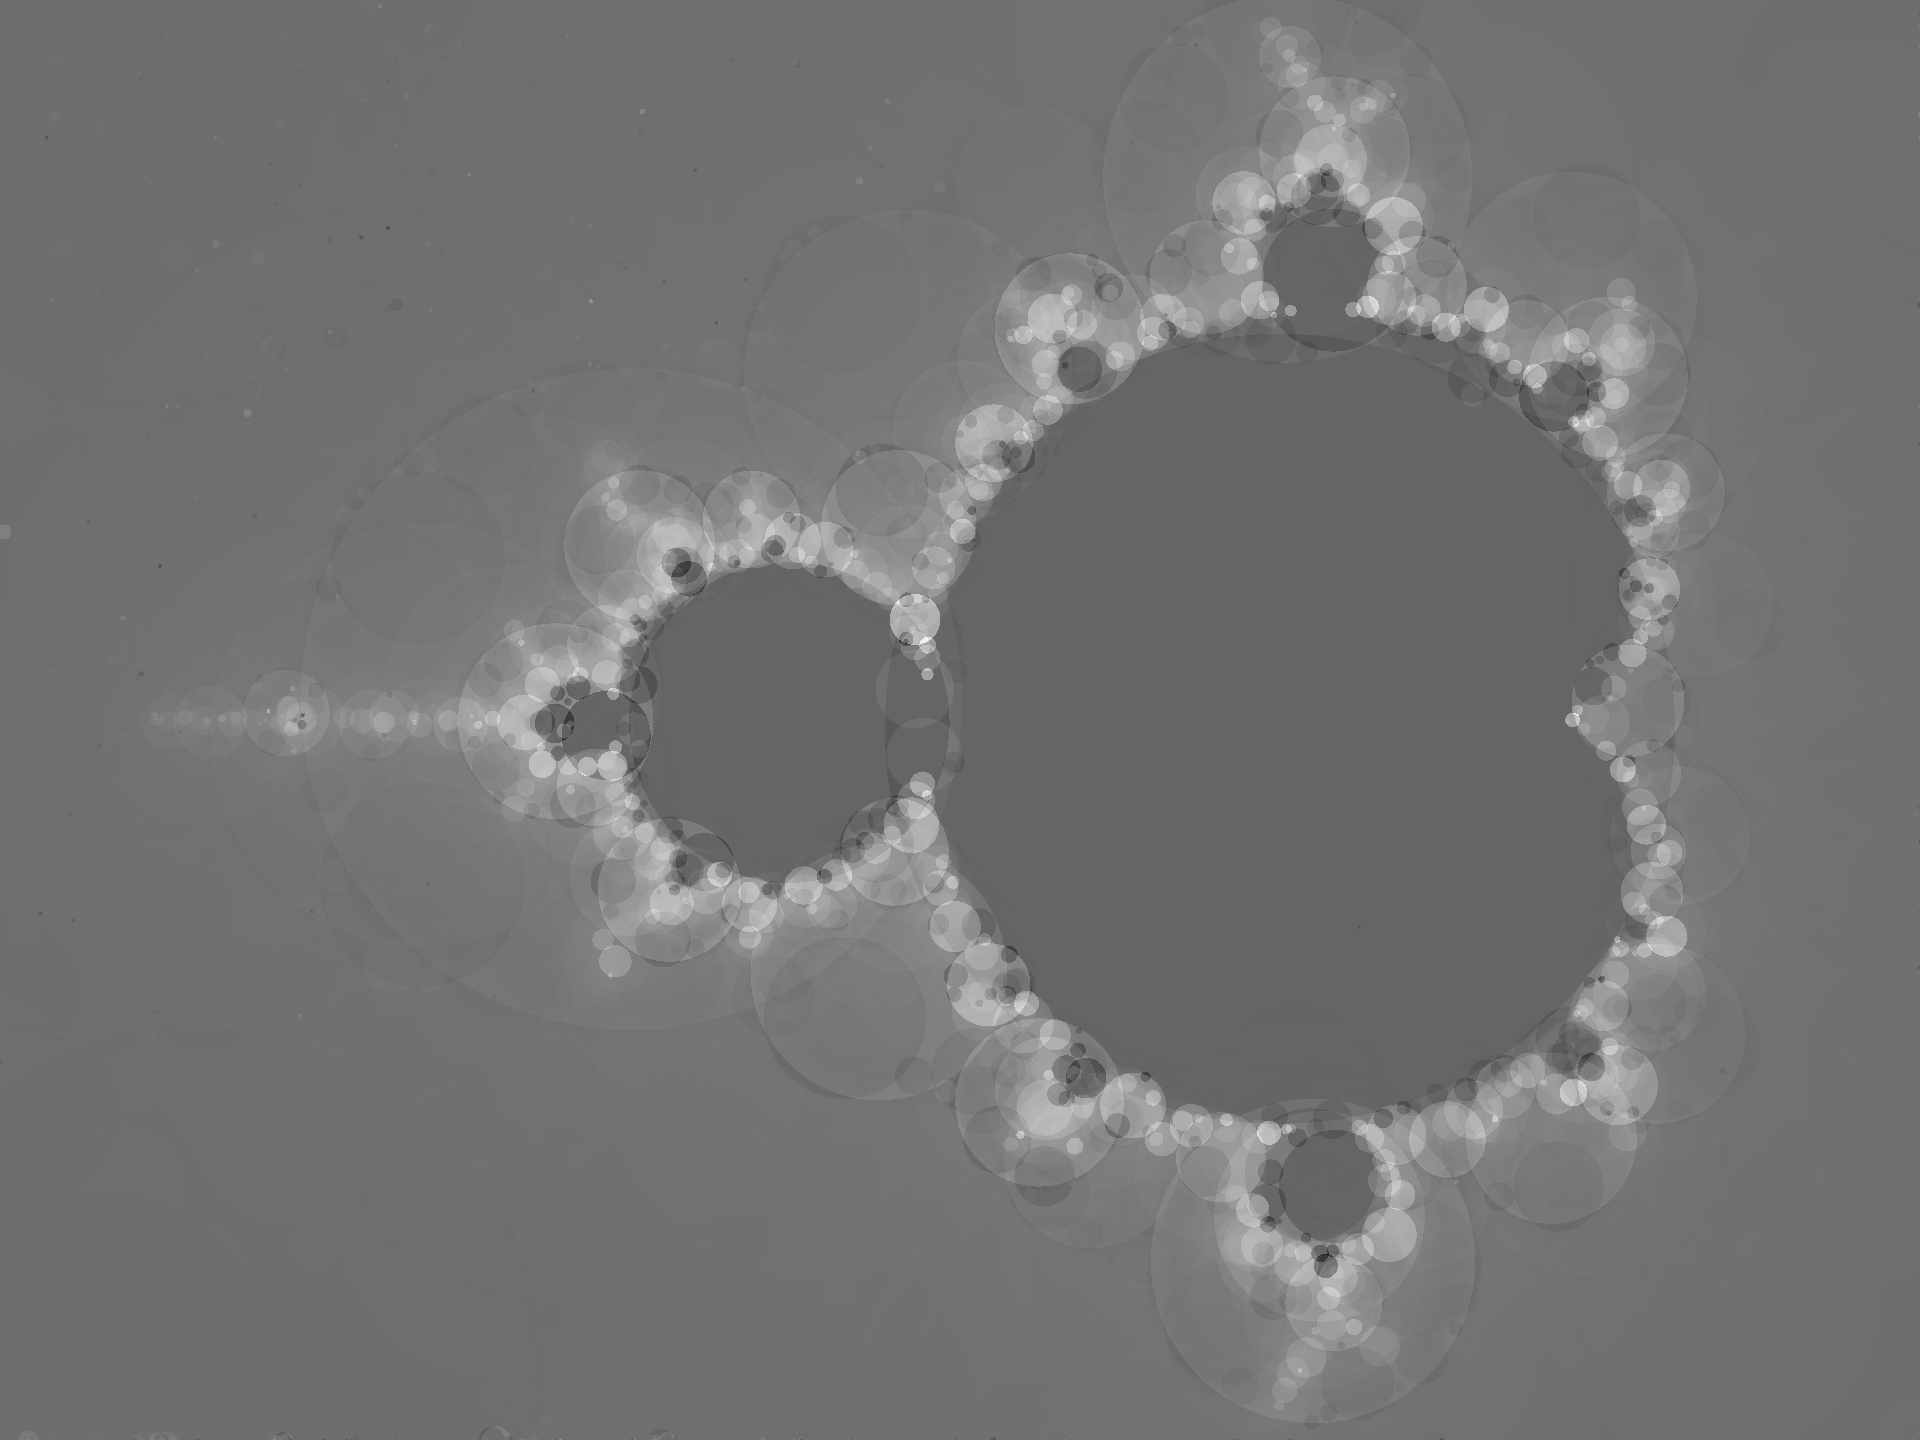
\includegraphics[width=0.75\textwidth]{../results/mandlebrot/mandlebrot_raw_wrong_4000}
\caption{Mandlebrot Set at 1920x1440 resolution}
\label{fig:mandlebrot_raw}
\end{figure}

Having now had a half-semester to digest and process information about nature-inspired computing approaches like simulated annealing and various implementations of evolutionary algorithms, Homework \#2 challenged us to tackle a nontrivial task: image reproduction. Our official bidding was to use an evolutionary algorithm (with our own quirks)  to evolve the closest approximation of a given image. Our implementation focused on a very robust generation-to-generation reproduction system using both crossover and point mutations. This approach yielded remarkable results. 
\\ \\
\textbf{Note: }The repository for this paper can be found \href{https://github.com/macattackftw/ncGA}{here}. 
The \verb|README.md| contains several animations of our solution in action and a full suite of test results can be seen in the \verb|results| folder. A selection of these results can also be seen in Appendix A. 

%\section*{} %%  This will generate a numbered problem header.

\newpage
%%%%%%%%%%%%%%%%%%%%%%%%%%%%%%%%%%%%%%%%%%%%%%%%%%%%%%%%%%%%%%%%%%%%%%%%%%%%%%%
\section*{Initial Approach and Encoding}
Before programming could begin we needed to know \textbf{1)} the language with which we would write our project, and \textbf{2)} the exact algorithm we were implementing. Python was the obvious choice for quickly iterating and testing. Algorithm development started at the discussion of how exactly we were going to generate images. After some back and forth we decided to build our image reconstructions purely in grayscale, and with layered circles. One ``epoch'' would be completed to generate an optimal circle. Each epoch would consist of a \textit{uniform randomly} generated population which was to be evolved over a set number of generations, with the most fit individual pulled and added to the reconstruction. While computationally intensive this one-at-a-time approach was expected to be robust and consistently convergent. 
\\
Encoding the properties of a circle into a genome was quite simple. We used \verb|numpy| to define a datatype that held the following information:
\begin{itemize}
\item The circle's center coordinates, $(x, y)$
\item The circle's radius, $r$
\item the circle's intensity, or alpha value, $i$
\end{itemize}

The actual definition of our genome can be seen below:
\begin{minted}{python}
center = np.dtype([('x', np.float32), ('y', np.float32)])
genome = np.dtype([('center', self.center), ('radius', np.float32), ('intensity', np.float32)])
\end{minted}


%%%%%%%%%%%%%%%%%%%%%%%%%%%%%%%%%%%%%%%%%%%%%%%%%%%%%%%%%%%%%%%%%%%%%%%%%%%%%%%
\section*{Measuring Individual Fitness}
Given a circle to be placed on the stack of circles, how do we determine how "fit" this individual is relative to any other circle? This question plagued us for days. Unlike a simple mathematical function one can't just plug a circle into an image and get a numeric out indicating progress. The circle's fitness depends on not only the information confined to its bounds, but also how the circle fits into the larger context of the image. Our initial approaches to generating a fitness function proved fruitless; one simply filled the image as quickly as possible with white, and another would produce results only slightly better than random circle placement. 

We eventually determined that, given a circle, we should:
\begin{enumerate}
\item Determine the number of pixels occupied by the circle, $n$
\item Generate the circle in a mask
\item Add this mask to the current circle stack, constructing  a prospective next-circle stack
\item Determine the total difference between this prospective stack and the actual image to be reconstructed, $e$
\item Formulate a normalization factor, $p = n/(total pixel count)$
\item Return a final fitness $e - p$
\end{enumerate}

This is a minimization process. The best circles will be ones that have a zero sum difference $e$. To differentiate between equal $e$ values we subtracted $p$ to give larger circles a very slight advantage. The advantage was kept at $<= 1$ so that it would only impact circles of equivalent $e$ values.
\\

Our fitness function definition is as follows:

\begin{minted}{python}
def Fitness(self, individual):
  # Calculate mask
  cx, cy, r = individual['center']['x'], individual['center']['y'], individual['radius']
  Y, X = np.ogrid[-cy:self.height - cy, -cx:self.width - cx]
  mask = X**2 + Y**2 <= r**2                
  
  # Gen prospective stack
  circle_pixels = np.sum(mask, dtype=np.float32)
  circle = mask * individual['intensity']
  art = self.art + circle

  return np.sum(np.abs(self.image - art)) - circle_pixels / self.pixel_count
\end{minted}

This fitness function tracks how well the circle improved its local area relative to its size. Once we had it in place, the stars aligned and things converged!

%%%%%%%%%%%%%%%%%%%%%%%%%%%%%%%%%%%%%%%%%%%%%%%%%%%%%%%%%%%%%%%%%%%%%%%%%%%%%%%
\section*{Evolving a New Circle}
Our process of generating and selecting a new circle is somewhat involved. Each final circle is the product of a full evolutionary run with its own population. We followed a fairly standard approach:

$$
\textit{initialize population}
\rightarrow\textit{evaluate fitness}
\rightarrow\textit{crossover/mutate}
\rightarrow\textit{breed next generation}
$$

\subsection*{Mutation and Crossover}
Our crossover implementation is as simple as it gets: take two individuals and calculate the average $x$ and $y$ center positions, the radii, and the intensity. The mutation process takes into account how many generations have been evolved up to that point and uses a step function to determine what the normal distribution's $\mu$ and $\sigma$ should be. For each attribute $a$ of the circle to mutate:

\begin{enumerate}
\item Generate a Gaussian random number $p$ using $\mu, \sigma$
\item Determine a proportional shift $\tilde{a} = p*a$
\item Calculate the new, mutated value $a^{\prime} = a + \tilde{a}$
\item Set $a = a^{\prime}$ 
\end{enumerate}
The distribution deviation $\sigma$ changes depending on generation count. For the first three generations $\sigma = 0.3$, for generations in the first half after the first three $\sigma = 0.2$, and for the last half of the generations $\sigma = 0.1$. This has the effect of tapering off the magnitude of mutation variations as generation count increases and, hopefully, the individuals home in on local maxima. Simulated annealing can work alongside GAs!

We also implemented another mutation strategy for a specific case to be discussed later. This takes in a circle and explicitly mutates each attribute in both an increasing \textit{and} decreasing direction.


\subsection*{Selection and Generation}
The approach we've taken to population evolution is a bit more complicated than ranked selection and breeding. 

There are four distinct categories for selection:
\begin{enumerate}
    \item Royalty survive
    \item Royalty breed with commoner
    \item Everyone has a chance to breed
    \item Most fit undergoes inbreeding
\end{enumerate}

Given a population ranked by fitness we select a top proportion (the ``Royalty'') to survive into the next generation. This is defined by the \texttt{ELITISM} class member. Then we perform what we call \texttt{Cinderella Selection} in which a random member of the Royalty will breed with a commoner. This produces two children:
\begin{enumerate}
    \item An averaging of the parents
    \item A mutation of the average
\end{enumerate}

The next selection step is random chance, where any member could breed with any other member. In particularly small populations it is possible this will be a duplicate of a previous arrangement. And in the final step we take the most fit (``Best'') individual and perform inbreeding, Habsburg-style. The Best undergoes a positive and negative mutation to each of the three categories:
\begin{itemize}
    \item Center
    \item Radius
    \item Intensity
\end{itemize}

Since this is the best we do not wish to stray too far from where we currently are, therefore for positive mutations we see $\mu = 0.1$ and $\sigma = 0.1$, while for negative mutations we see $\mu = -0.1$ and $\sigma = 0.1$. This slightly offsets the normal distribution so a small change is effected to each of the six resulting offspring.


%%%%%%%%%%%%%%%%%%%%%%%%%%%%%%%%%%%%%%%%%%%%%%%%%%%%%%%%%%%%%%%%%%%%%%%%%%%%%%%
\section*{Results}
The algorithm described in the above sections functioned stupendously well. In initial testing it became clear even with small circle counts that the algorithm was converging quickly to reconstructions that contained core structural information of the original images. Figure \ref{fig:darwin_0050} shows this early tendency towards low-frequency, high-gain information clearly. As circle counts increased high-frequency information started appearing, with massive circle counts almost identical to the original image. Over a dozen examples of high-count reconstructions can be found in Appendix A. 
\begin{figure}[H]
\centering
\noindent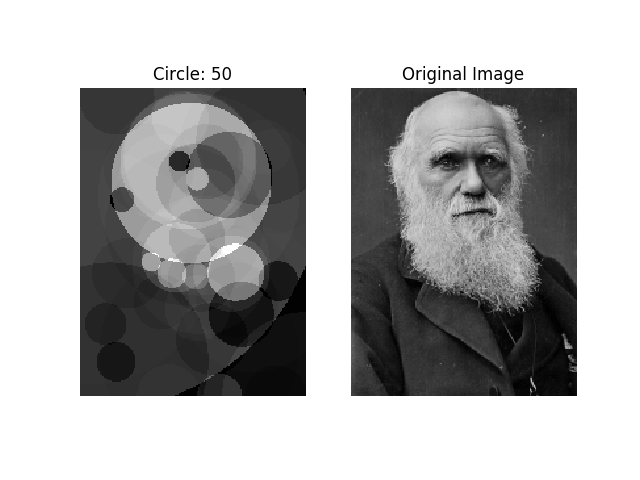
\includegraphics[width=0.4\textwidth]{../results/darwin/darwin_0050}
\noindent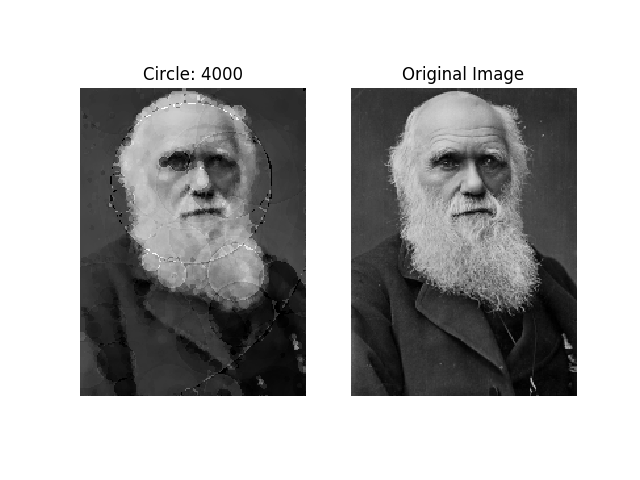
\includegraphics[width=0.4\textwidth]{../results/darwin/darwin_4000}
\caption{A portrait of Charles Darwin with 50 and 4000 circles, respectively. }
\label{fig:darwin_0050}
\end{figure}

There are some cases where the algorithm does not perform as well as expected. One case is that of cartoon characters: large swaths of empty space punctuated by very sharp, thin lines and hard gradients. Such information proved difficult for circles to represent using low circle counts. However, given a truly massive number of elements and time to work with, the algorithm did manage to reconstruct drawings satisfactorily. Figure \ref{fig:hobbes_0200} demonstrates this behavior well. 
\begin{figure}[H]
\centering
\noindent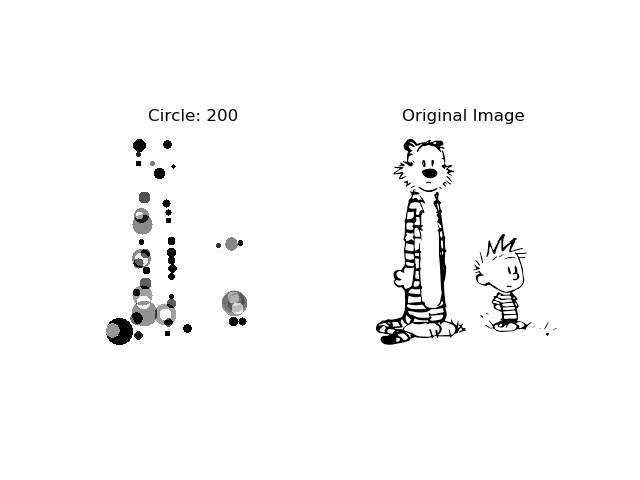
\includegraphics[width=0.4\textwidth]{../results/cartoons/hobbes_0200}
\noindent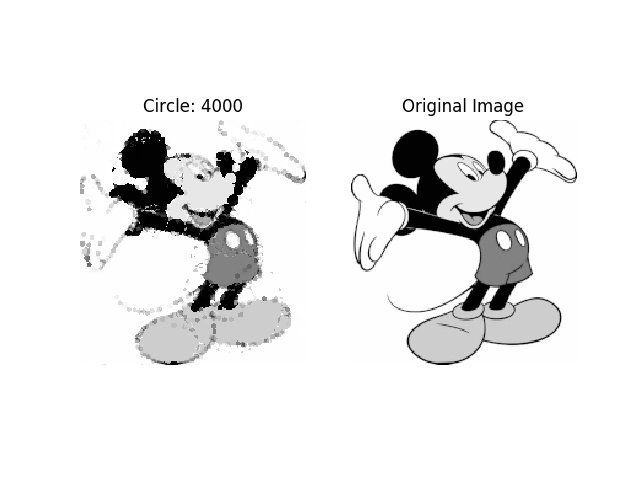
\includegraphics[width=0.4\textwidth]{../results/mickey/mickey_4000}
\caption{Cartoon/comic drawings reconstructed. }
\label{fig:hobbes_0200}
\end{figure}

Curiously, our initial expectations about larger populations leading to faster convergence were incorrect. In testing (shown in Figure \ref{fig:lenna_pop}) we found that there was little practical value to a population size greater than 25. Increasing population size does appear to increase the prevalence of large circles, and the circles seem to be more "correctly" placed on average. 
\begin{figure}[H]
\centering
\noindent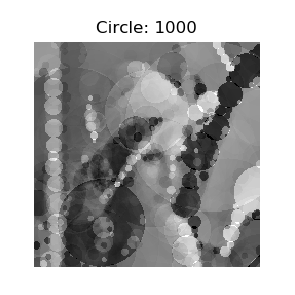
\includegraphics[width=\textwidth/6]{../results/lenna/lenna_pop10}
\noindent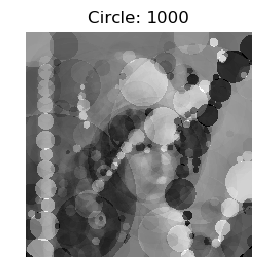
\includegraphics[width=\textwidth/6]{../results/lenna/lenna_pop20}
\noindent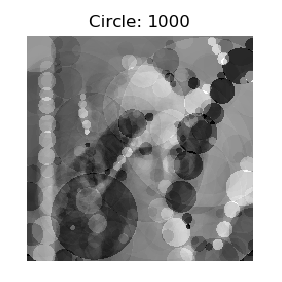
\includegraphics[width=\textwidth/6]{../results/lenna/lenna_pop28}
\noindent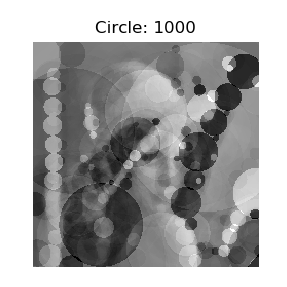
\includegraphics[width=\textwidth/6]{../results/lenna/lenna_pop35}
\noindent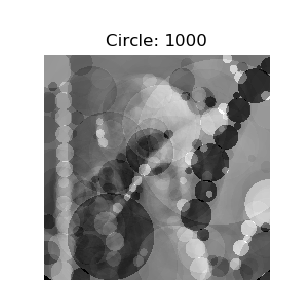
\includegraphics[width=\textwidth/6]{../results/lenna/lenna_pop50}
\caption{Images generated with 1000 circles, 100 generations, and population size = (10, 20, 28, 35, 50). }
\label{fig:lenna_pop}
\end{figure}

Being astute students, we also varied generation count to see what effect it would have on reconstruction quality. Holding at a constant population size of 20 individuals and varying the generation count from 25 to 200 we really didn't see drastic changes. Figure \ref{fig:lenna_gen} shows these results. There is an increase in feature clarity as generation count increases, but one would be hard-pressed to find a fundamental difference between the images generated with 50 generations and 200 generations. 
\begin{figure}[H]
\centering
\noindent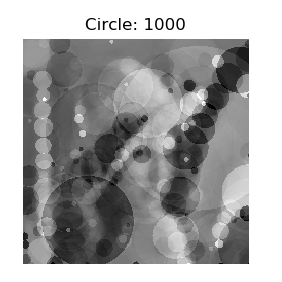
\includegraphics[width=\textwidth/6]{../results/lenna/lenna_gen25}
\noindent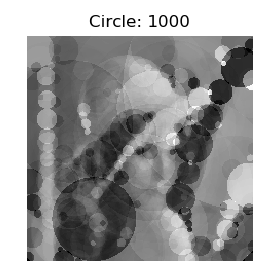
\includegraphics[width=\textwidth/6]{../results/lenna/lenna_gen50}
\noindent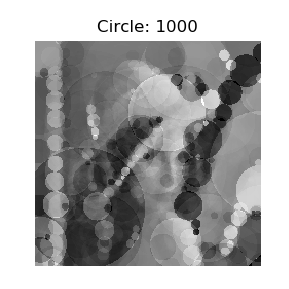
\includegraphics[width=\textwidth/6]{../results/lenna/lenna_gen75}
\noindent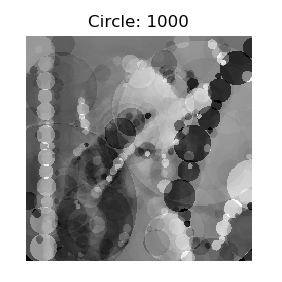
\includegraphics[width=\textwidth/6]{../results/lenna/lenna_gen100}
\noindent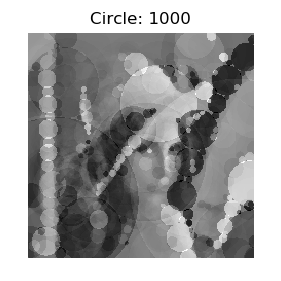
\includegraphics[width=\textwidth/6]{../results/lenna/lenna_gen200}
\caption{Images generated with 1000 circles, population of 20, and generation count = (25, 50, 75, 100, 200). }
\label{fig:lenna_gen}
\end{figure}

With the above testing we can arrive at a practical optimization of 25-30 individuals, 50 generations. Using 28 individuals and 50 generations produced the below image (Figure \ref{fig:lenna_final}) in 7 minutes, 25 seconds on an i7 2600k CPU from 2011. 
\begin{figure}[H]
\centering
\centering
\noindent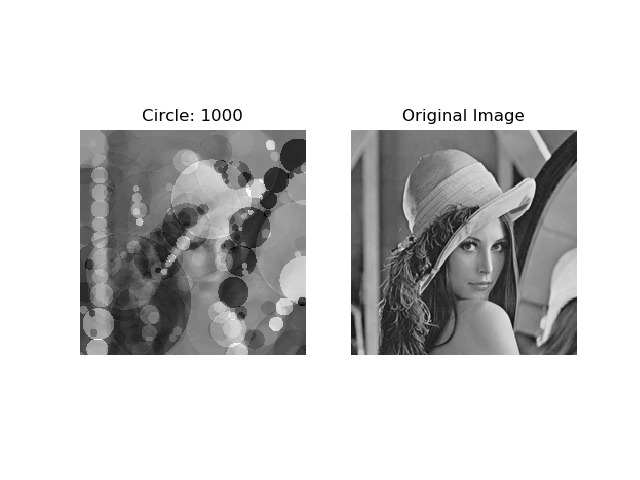
\includegraphics[width=0.75\textwidth]{../results/lenna/lenna_pop28_gen50}
\caption{Roughly-optimized generation of 1000 circles, population size = 28, generations = 50.}
\label{fig:lenna_final}
\end{figure}

Learning that the population size can be relatively small we tested the limits of what we could approximate utilizing only 4,000 cirlces. We ran an image of the Mandlebrot Set with 2,764,800 pixels (1920 x 1440 resolution) and an image of Old Glory with 3,368,160 pixels (2339 x 1440 resolution) as can be seen in Figures \ref{fig:mandlebrot} and \ref{fig:old_glory} respectively. The resulting images follow the ``across the room`` effect that we noticed in the earlier runs. This effect was first noticed when observing thumbnails for the images. The thumbnails of the generated images appear very similar to the original image but when you open the generated image there is a very clear distinction. This effect can be seen between Figures \ref{fig:mandlebrot} and \ref{fig:mandlebrot_raw}.

The stack of circles we identified as \texttt{self.art}. We knew it was possible for the image to have values outside of the \texttt{[0, 255]} range since we allowed for circles to just layer over the existing art. This freedom is what allowed for the image to have darkened areas. It would have been possible to test if capping per epoch (circle drawn) would have an impact on the overall art but we did not have time to test that. You can see the difference between what our art was and what we saved by looking at Figures \ref{fig:mandlebrot_raw_wrong} and \ref{fig:mandlebrot_raw} respectively. The range on Figure \ref{fig:mandlebrot_raw_wrong} was \texttt{(-250.501, 383.776)}.

%%%%%%%%%%%%%%%%%%%%%%%%%%%%%%%%%%%%%%%%%%%%%%%%%%%%%%%%%%%%%%%%%%%%%%%%%%%%%%%
\section*{Conclusions}
Perhaps unsurprisingly, we discovered that robust genetic algorithms work well to (eventually) reproduce images from primitive shapes. The importance of a good fitness function was also very apparent after a couple days working on this project. We spent several days attempting to tune the fitness function and once we tuned it the rest of the algorithm just worked. This project has handily showed that evolutionary algorithms are very capable tools (when corralled correctly) for solving problems without a hard mathematical definition. 

%%%%%%%%%%%%%%%%%%%%%%%%%%%%%%%%%%%%%%%%%%%%%%%%%%%%%%%%%%%%%%%%%%%%%%%%%%%%%%%
\section*{Future Work}
Our results showed this to be a very effective means of approximating an image. Run times on images is prohibitively long and one approach to rectify that could be implementation of multithreaded or distributed solutions. Another area for exploration is introducing colored circles. We found the algorithm to be extremely robust to fluxuations in population and generation sizes so it is reasonable to assume it would perform well with a slightly larger population and RGB circles. During testing we observed the best and worst fitness for each generation. When generating random numbers we found that depending on the $\sigma$ allowed the fitness tended to converge around a certain generation. Future work could involve a dynamic generation, where it progresses until the change between generations is within $\epsilon$ and then it would move on to the next epoch. Lastly, the methodology is sound, so this should work for \textit{any} geometric shape. Allowing user to decide the geometric shape would be a good expansion on this work.


\newpage
%%%%%%%%%%%%%%%%%%%%%%%%%%%%%%%%%%%%%%%%%%%%%%%%%%%%%%%%%%%%%%%%%%%%%%%%%%%%%%%
\section*{Appendix A: Reconstructed Images}

\subsection*{Low Resolution}
\begin{figure}[H]
\centering
\noindent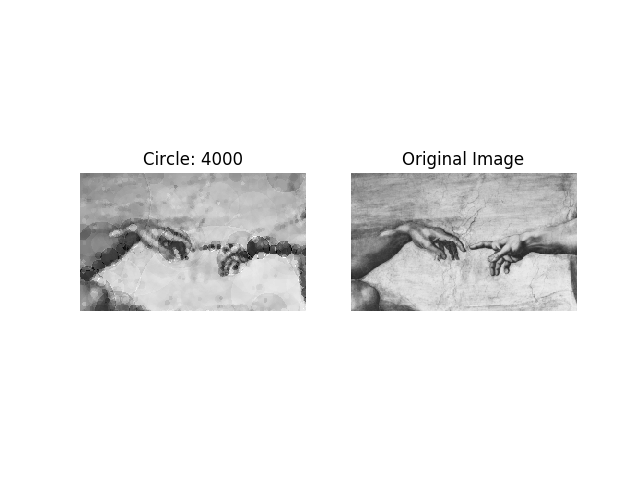
\includegraphics[width=0.75\textwidth]{../results/adam/adam_4000}
\caption{\textit{Creation of Adam} at 245 x 150 resolution}
\end{figure}

\begin{figure}[H]
\centering
\noindent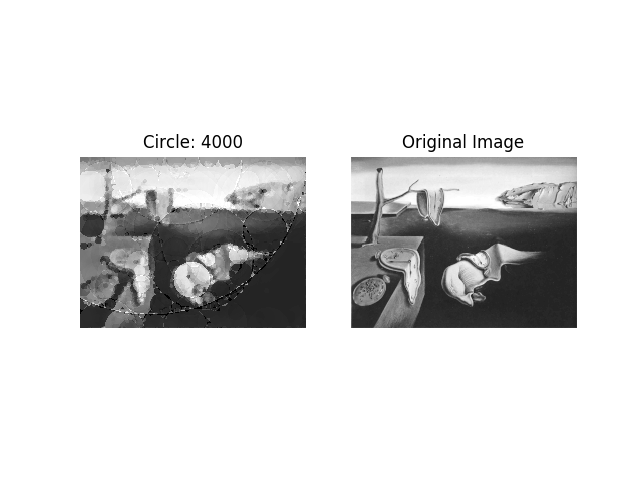
\includegraphics[width=0.75\textwidth]{../results/dali/dali_4000}
\caption{\textit{The Persistence of Memory} at 225 x 171 resolution}
\end{figure}

\begin{figure}[H]
\centering
\noindent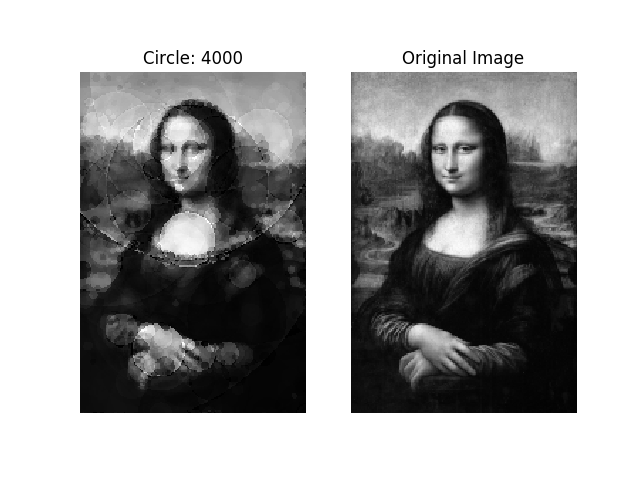
\includegraphics[width=0.75\textwidth]{../results/mona_lisa/mona_lisa_4000}
\caption{\textit{Mona Lisa} at 159 x 240 resolution}
\end{figure}

\begin{figure}[H]
\centering
\noindent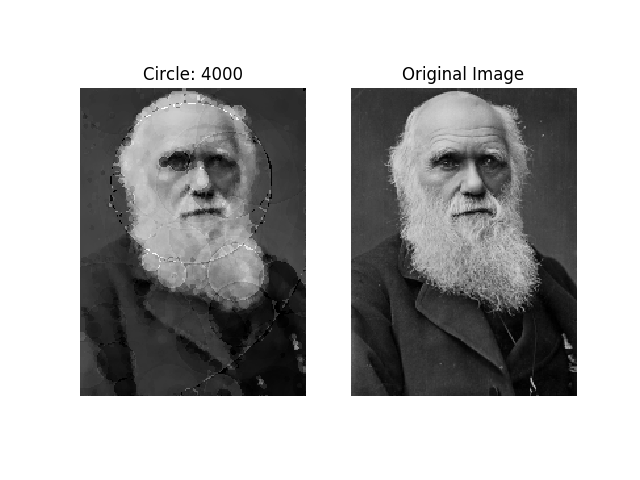
\includegraphics[width=0.75\textwidth]{../results/darwin/darwin_4000}
\caption{Charles Darwin at 172 x 235 resolution}
\end{figure}

\begin{figure}[H]
\centering
\noindent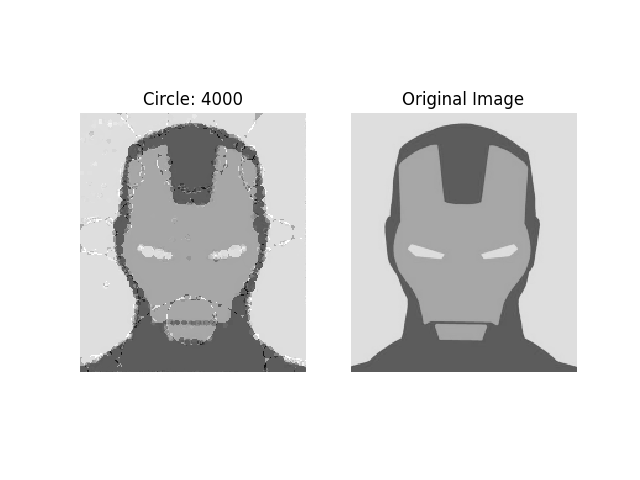
\includegraphics[width=0.75\textwidth]{../results/ironman/ironman_4000}
\caption{Iron Man at 183 x 210 resolution}
\end{figure}

\begin{figure}[H]
\centering
\noindent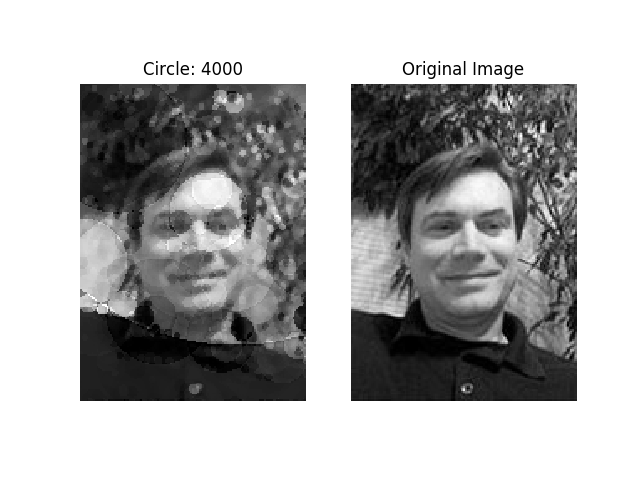
\includegraphics[width=0.75\textwidth]{../results/jmcgough/jmcgough_4000}
\caption{Jeff McGough at 135 x 190 resolution}
\end{figure}

\begin{figure}[H]
\centering
\noindent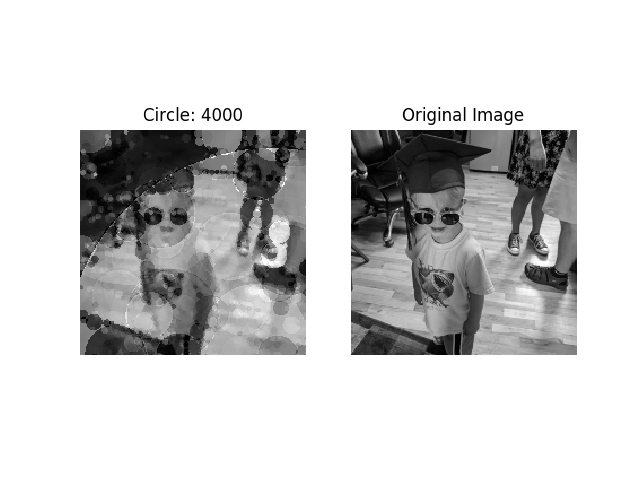
\includegraphics[width=0.75\textwidth]{../results/k/k_4000}
\caption{k at 200 x 200 resolution}
\end{figure}

\begin{figure}[H]
\centering
\noindent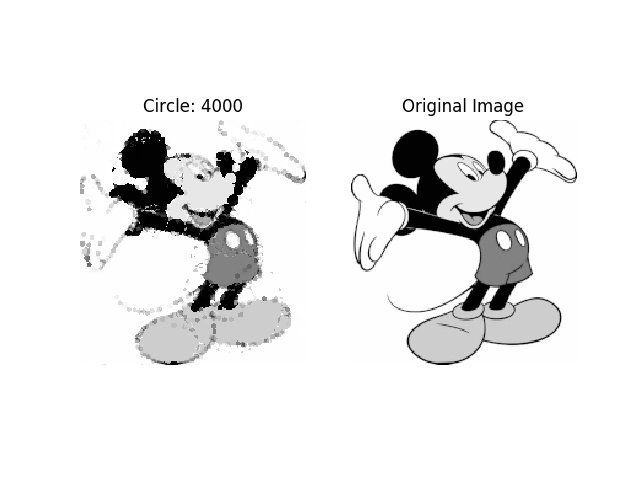
\includegraphics[width=0.75\textwidth]{../results/mickey/mickey_4000}
\caption{Mickey Mouse at 184 x 200 resolution}
\end{figure}


\begin{figure}[H]
\centering
\noindent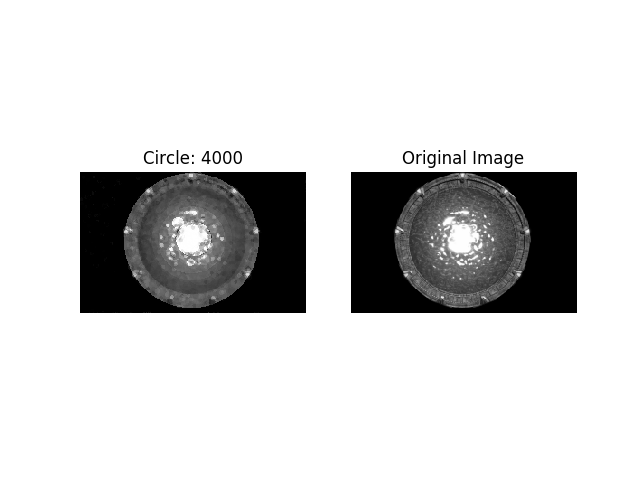
\includegraphics[width=0.75\textwidth]{../results/stargate/stargate_4000}
\caption{Stargate at 250 x 156 resolution}
\end{figure}

\begin{figure}[H]
\centering
\noindent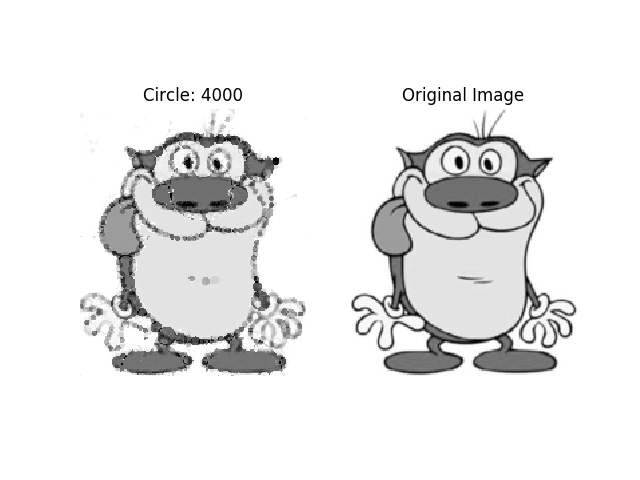
\includegraphics[width=0.75\textwidth]{../results/stimpy/stimpy_4000}
\caption{Stimpy at 169 x 200 resolution}
\end{figure}

\begin{figure}[H]
\centering
\noindent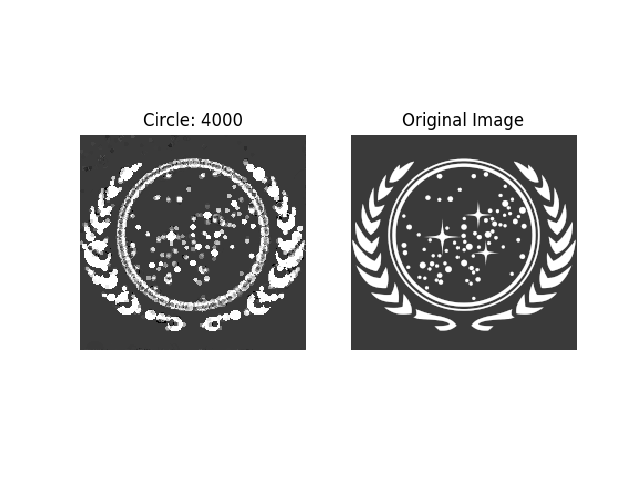
\includegraphics[width=0.75\textwidth]{../results/ufop/ufop_4000}
\caption{United Federation of Planets at 204 x 195 resolution}
\end{figure}



\newpage
\subsection*{Medium Resolution}
\begin{figure}[H]
\centering
\noindent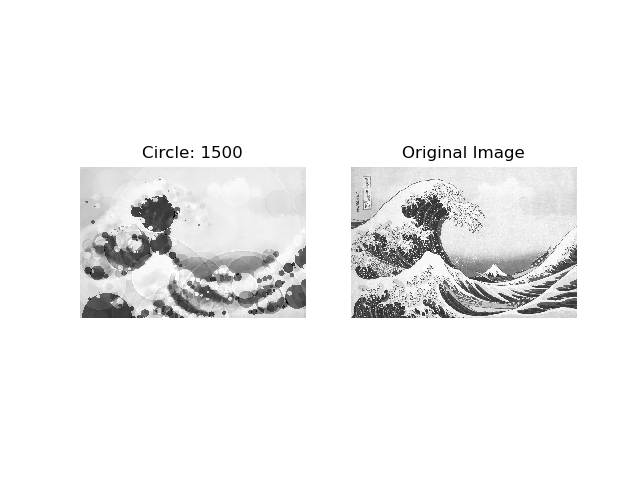
\includegraphics[width=0.75\textwidth]{../results/wave/wave_1500}
\end{figure}

\begin{figure}[H]
\centering
\noindent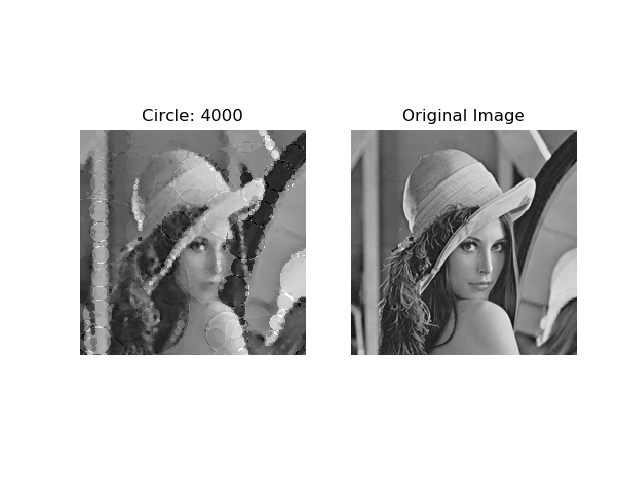
\includegraphics[width=0.75\textwidth]{../results/lenna/lenna_4000}
\end{figure}

\begin{figure}[H]
\centering
\noindent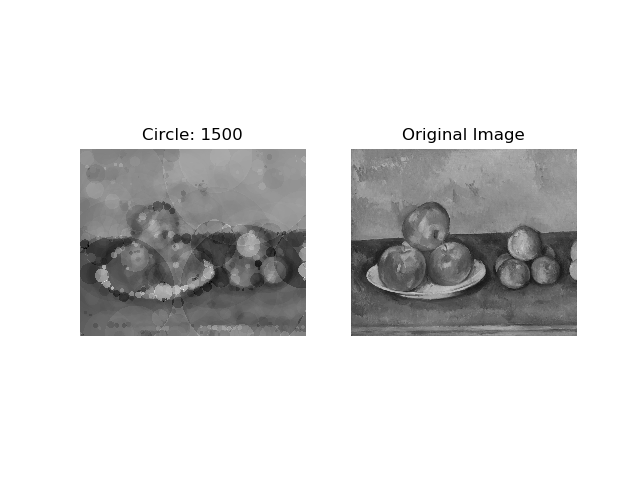
\includegraphics[width=0.75\textwidth]{../results/fruit/fruit2_1500}
\end{figure}

\begin{figure}[H]
\centering
\noindent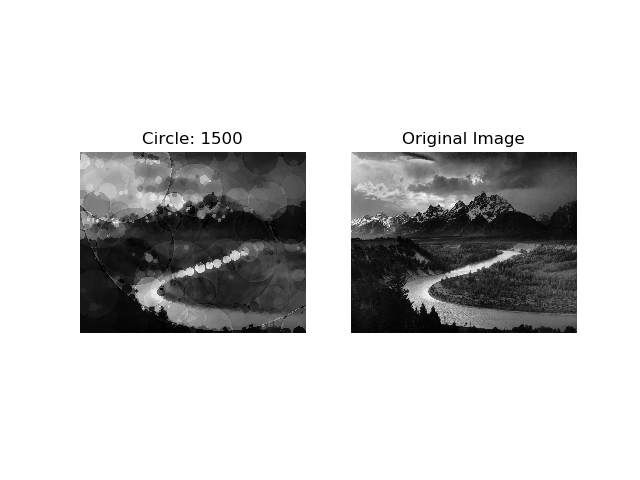
\includegraphics[width=0.75\textwidth]{../results/ansel/tetons_1500}
\end{figure}


\newpage
\subsection*{High Resolution}
\begin{figure}[H]
\centering
\noindent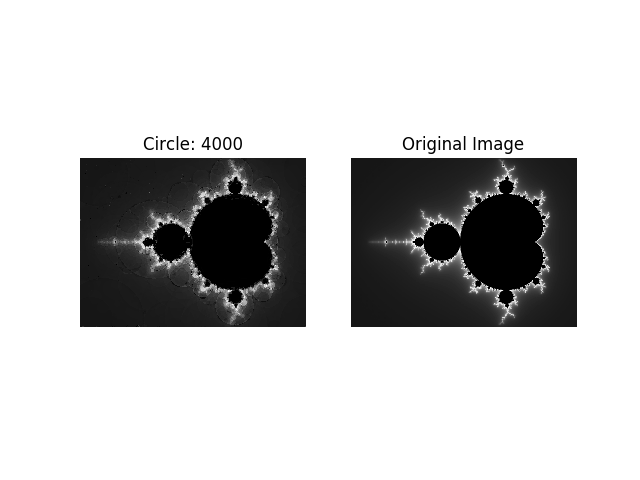
\includegraphics[width=0.75\textwidth]{../results/mandlebrot/mandlebrot_4000}
\caption{Mandlebrot Set at 1920x1440 resolution}
\label{fig:mandlebrot}
\end{figure}

\begin{figure}[H]
\centering
\noindent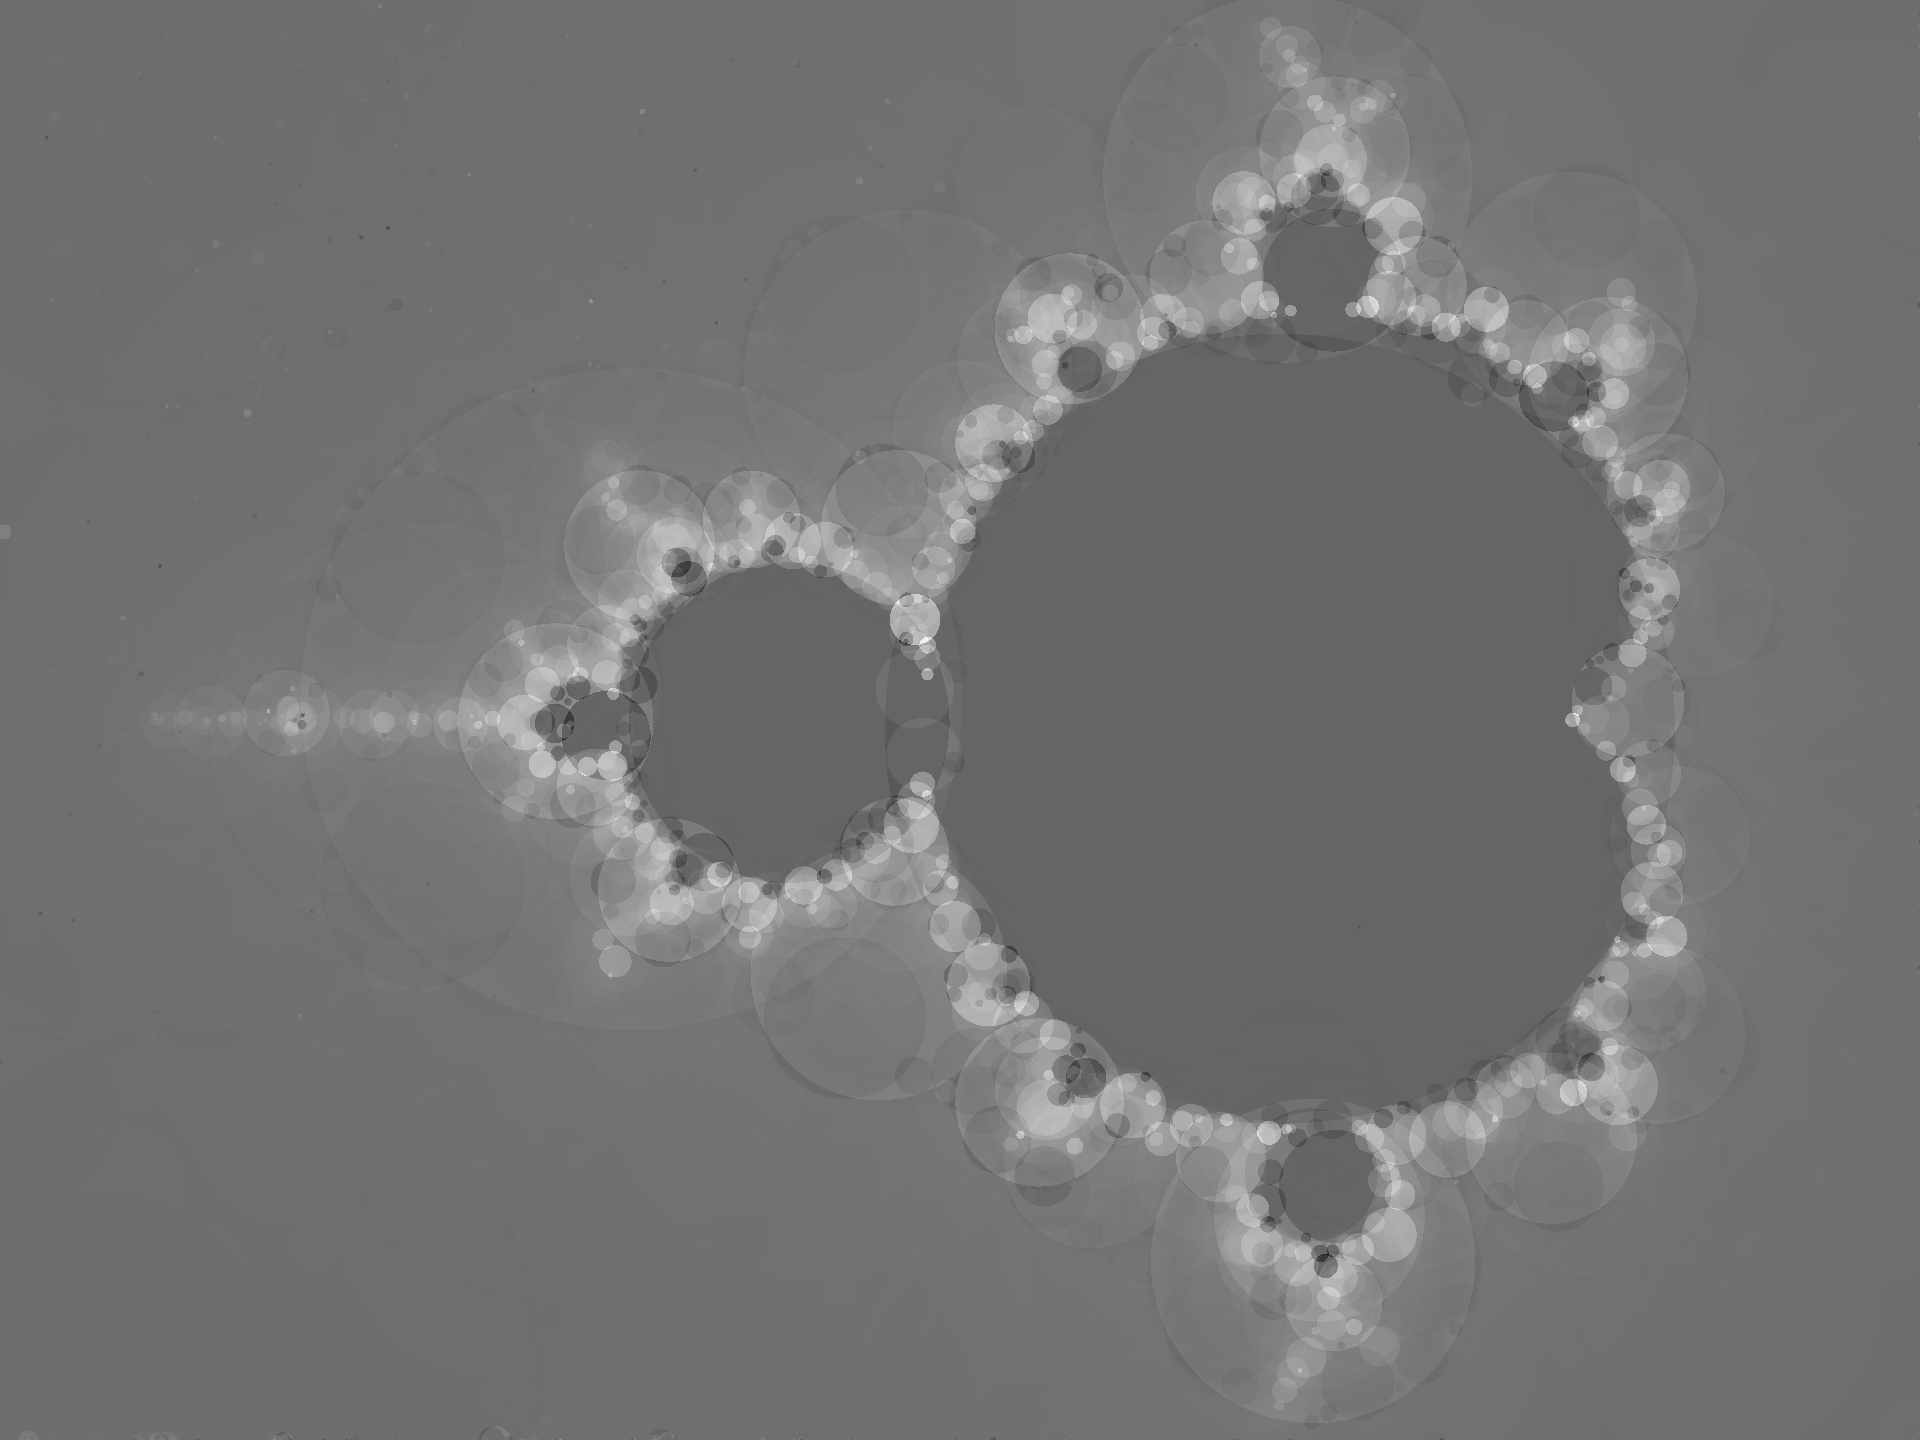
\includegraphics[width=0.75\textwidth]{../results/mandlebrot/mandlebrot_raw_4000}
\caption{Mandlebrot Set at full resolution}
\label{fig:mandlebrot_raw}
\end{figure}

\begin{figure}[H]
\centering
\noindent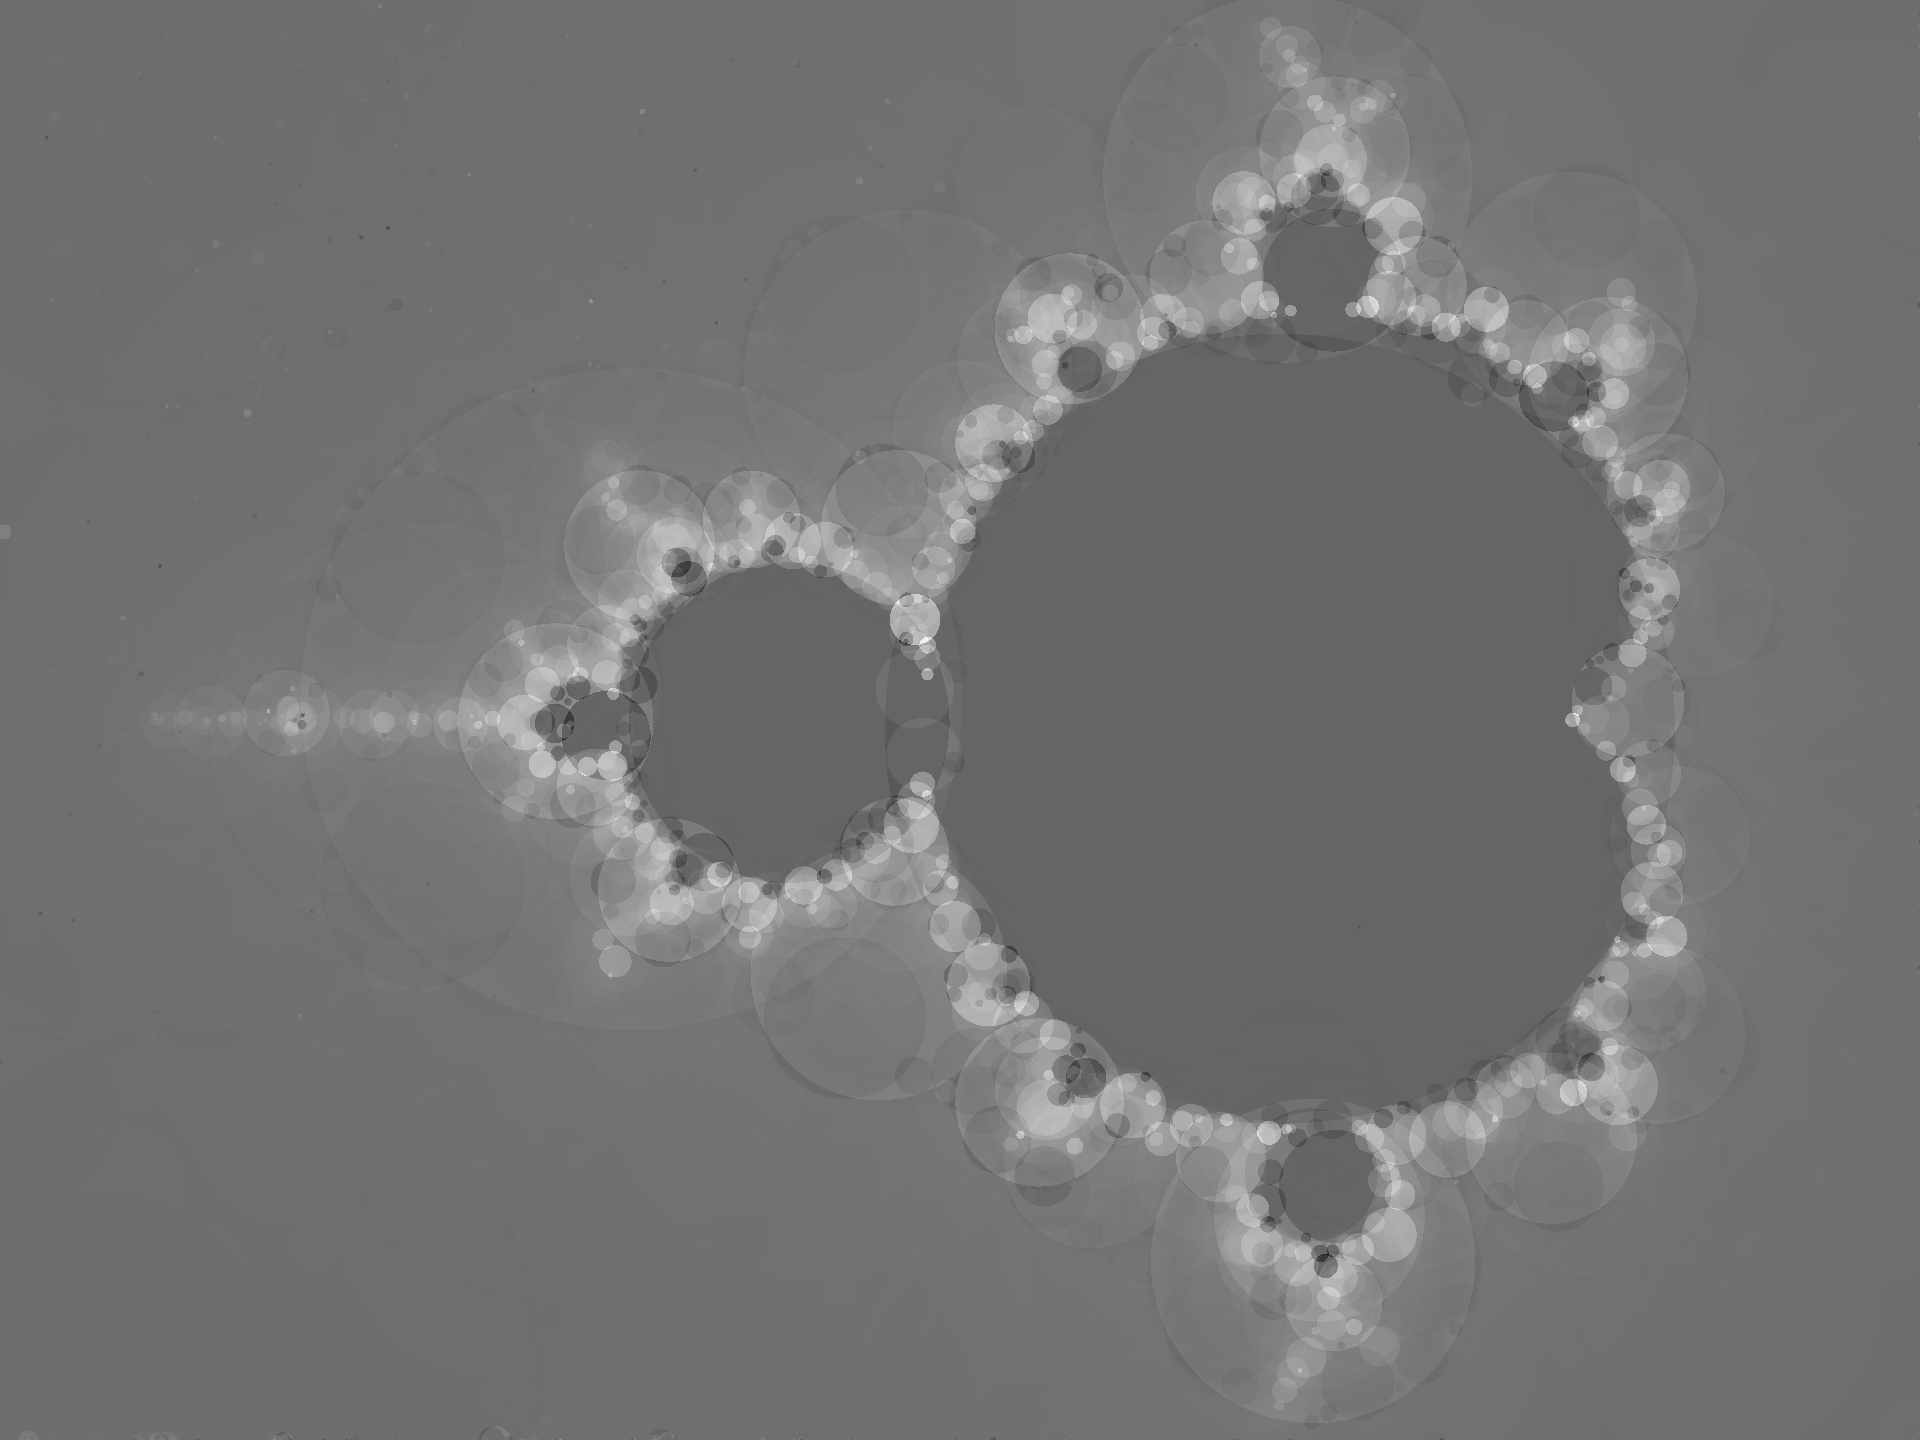
\includegraphics[width=0.75\textwidth]{../results/mandlebrot/mandlebrot_raw_wrong_4000}
\caption{Mandlebrot Set at full resolution}
\label{fig:mandlebrot_raw_wrong}
\end{figure}

\begin{figure}[H]
\centering
\noindent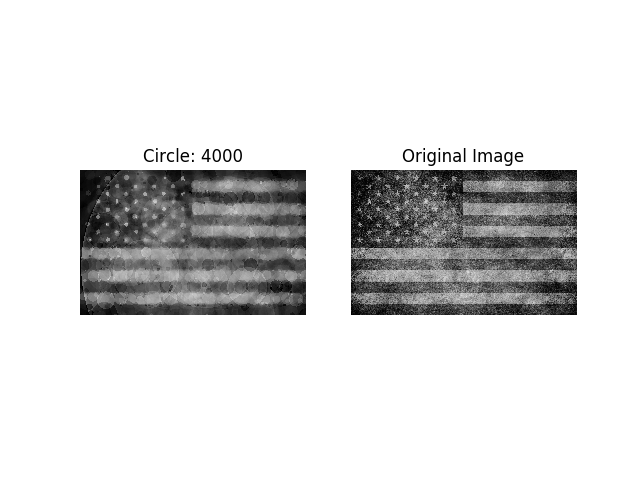
\includegraphics[width=0.75\textwidth]{../results/old_glory/old_glory_4000}
\caption{Old Glory at 2239x1440 resolution}
\label{fig:old_glory}
\end{figure}

% \begin{figure}[H]
% \centering
% \noindent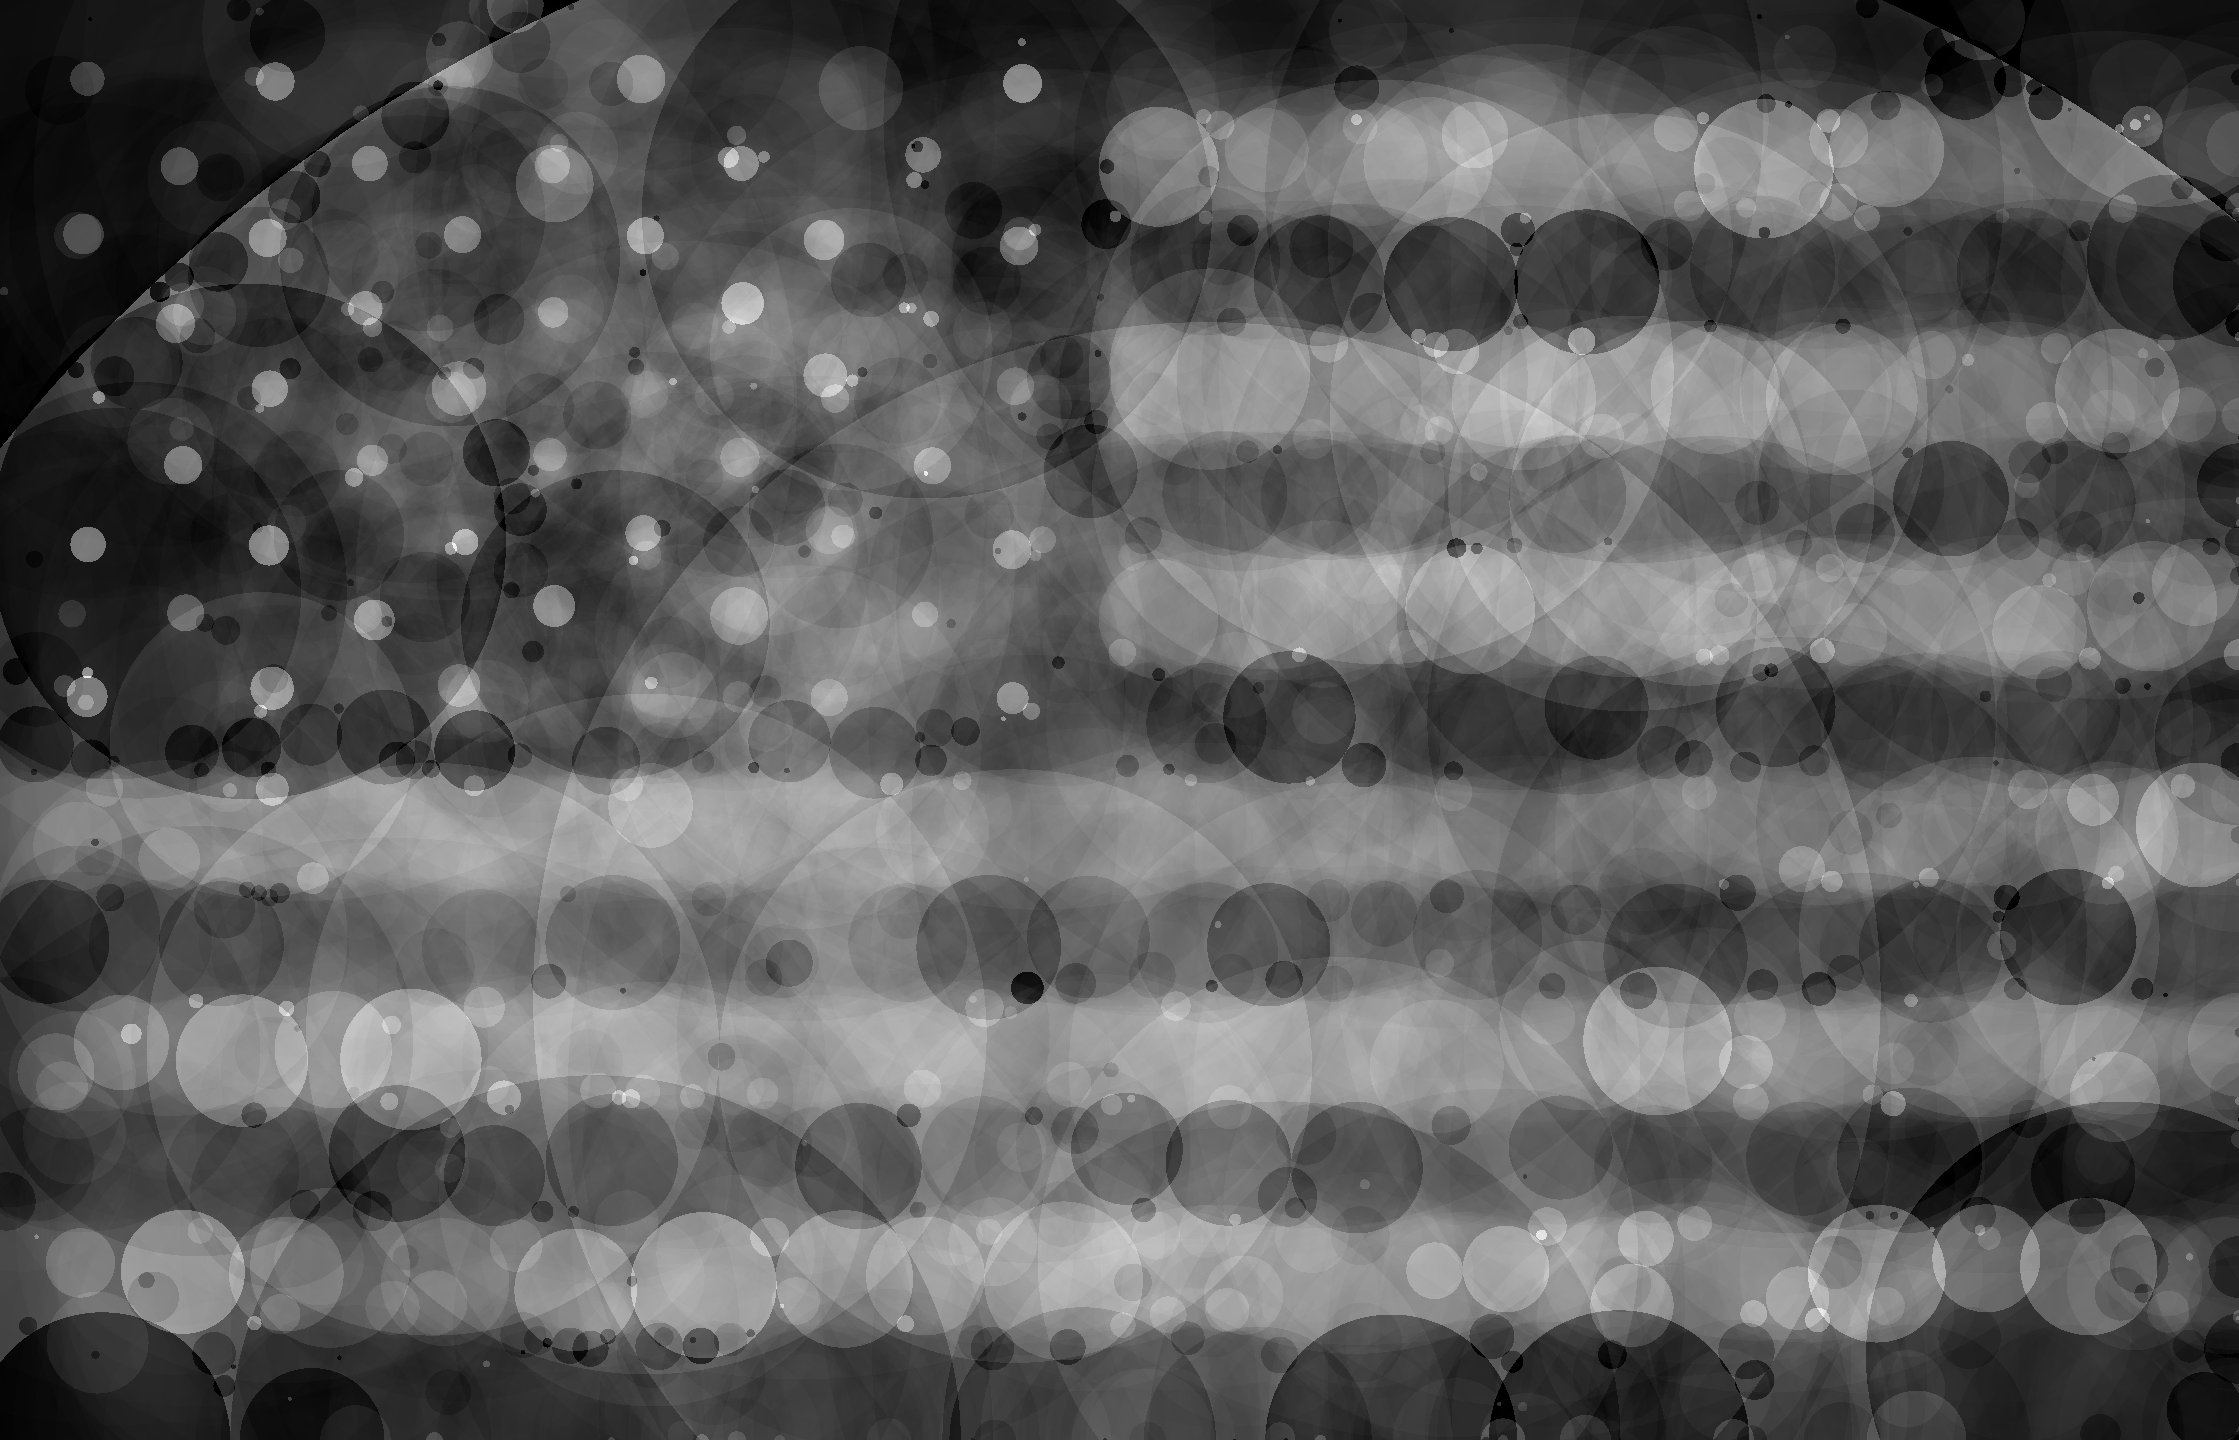
\includegraphics[width=0.75\textwidth]{../results/old_glory/old_glory_raw_4000}
% \caption{Old Glory at full resolution}
% \label{fig:old_glory_raw}
% \end{figure}






\newpage
\section*{Appendix B: Code}
\begin{minted}{python}
import numpy as np
import imageio
import matplotlib.pyplot as plt
from time import sleep, perf_counter
# import cProfile

class GA():
    ELITISM = 0.10
    def __init__(self, circles=4000, headless=False):
        self.epoch = 0
        self.SetPopAttributes()
        self.circles = circles
        self.center = np.dtype([('x', np.float32), ('y', np.float32)])
        self.genome = np.dtype([('center',self.center), ('radius', np.float32), ('intensity', np.float32) ])
        self.pop = np.zeros((self.pop_size, ), dtype=self.genome)
        self.headless = headless

    def SetPopAttributes(self):
        if self.epoch < 200:
            self.pop_size = 200
            self.gens = 200
        else:
            self.pop_size = 10
            self.gens = 50

    def Reset(self):
        self.img_fitness = 0
        self.epoch = 0

    def Run(self, image):
        """Run the Genetic Algorthm"""
        filename = image[7:len(image) - 4]
        self.LoadImage(image)
        self.Reset()
        while self.epoch < self.circles:
            self.SetPopAttributes()
            self.InitializePop()    # 1
            self.EvaluatePop()
            if not self.headless:
                self.Draw()

            for self.gen in range(self.gens):
                self.Breed()        # 2
                self.EvaluatePop()
            self.UpdateImage()

            # For each epoch draw only if headless. Print on 50/100/200
            if self.epoch == 0:
                if self.headless:
                    self.Draw()
            elif self.epoch == 49:
                if self.headless:
                    self.Draw()
                plt.savefig('results/' + filename + '_0050.png')
            elif self.epoch == 99:
                if self.headless:
                    self.Draw()
                plt.savefig('results/' + filename + '_0100.png')
            elif self.epoch == 199:
                if self.headless:
                    self.Draw()
                plt.savefig('results/' + filename + '_0200.png')
            elif self.epoch == 499:
                if self.headless:
                    self.Draw()
                plt.savefig('results/' + filename + '_0500.png')
            elif self.epoch == 999:
                if self.headless:
                    self.Draw()
                plt.savefig('results/' + filename + '_1000.png')
            elif self.epoch == 1999:
                if self.headless:
                    self.Draw()
                plt.savefig('results/' + filename + '_2000.png')
            elif self.epoch == 2999:
                if self.headless:
                    self.Draw()
                plt.savefig('results/' + filename + '_3000.png')
            elif self.epoch == 3999:
                if self.headless:
                    self.Draw()
                plt.savefig('results/' + filename + '_4000.png')
            self.epoch += 1

        # When done display final image
        if not self.headless:
            self.epoch -= 1
            self.Draw()
            sleep(10)


    def LoadImage(self, image):
        """Will load an image file into the format we need"""
        # self.image = np.invert(imageio.imread(image))
        self.image = np.array(imageio.imread(image), dtype=np.float32)
        # Account for images with 3 dimensions
        if len(self.image.shape) == 3:
            self.height, self.width, _ = self.image.shape
            # Apply grayscale...
        else:
            self.height, self.width = self.image.shape
        self.max_dim = np.float32(max(self.height, self.width))
        self.pixel_count = np.float32(self.height * self.width)
        self.art = np.zeros((self.height, self.width), dtype=np.float32)
        self.max_radius = self.max_dim / 2.0

# 1
    def InitializePop(self):
        """Initialize pop"""
        self.rand_x = np.random.uniform(low=0,
                                        high=self.width - 1,
                                        size=self.pop_size)
        self.rand_y = np.random.uniform(low=0,
                                        high=self.height - 1,
                                        size=self.pop_size)
        self.rand_r = np.random.uniform(low=2.0,
                                        high=self.max_radius,
                                        size=self.pop_size)
        self.rand_i = np.random.uniform(low=-255.0,
                                        high=255.0,
                                        size=self.pop_size)
        for i in range(self.pop_size):
            self.pop[i] = self.FillGenomes(i)
        self.fitness = np.zeros(self.pop_size, dtype=np.float32)

    def FillGenomes(self, i):
        """Generates a genome"""
        center = np.array((self.rand_x[i], self.rand_y[i]), dtype=self.center)
        return np.array((center, self.rand_r[i], self.rand_i[i]),
                        dtype=self.genome)

    def EvaluatePop(self):
        """Evaluates each individual and sorts them"""
        for i in range(self.pop_size):
            self.fitness[i] = self.Fitness(self.pop[i])
        # Sort
        self.sorted_fitness = np.argsort(self.fitness)

    def Fitness(self, individual):
        """Scores fitness for an individual"""

        # https://stackoverflow.com/a/44874588/5492446 + Austin
        cx, cy, r = individual['center']['x'], individual['center']['y'], individual['radius']
        Y, X = np.ogrid[-cy:self.height - cy, -cx:self.width - cx]
        mask = X**2 + Y**2 <= r**2

        # Where the magic begins
        circle_pixels = np.sum(mask, dtype=np.float32)
        circle = mask * individual['intensity']
        art = self.art + circle

        return np.sum(np.abs(self.image - art)) - circle_pixels / self.pixel_count

# 2
    def Breed(self):
        """Selection and Crossover to generate a new population"""
        new_pop = np.zeros((self.pop_size, ), dtype=self.genome)

        # Take the most fit and keep them
        royalty = int(self.pop_size * GA.ELITISM)
        for i in range(royalty):
            pop_idx = self.sorted_fitness[i]
            new_pop[i] = np.copy(self.pop[pop_idx])

        # Have the most fit breed with the rest of the population
        royal_kids = 0
        while royal_kids < royalty:
            a, b = self.CinderellaSelection(royalty)
            c1, c2 = self.Crossover(a, b)
            new_pop[royal_kids + royalty] = c1
            royal_kids += 1
            if royal_kids < royalty:
                # Drop mutation if we're full
                new_pop[royal_kids + royalty] = c2
                royal_kids += 1

        # Fill the remainder of the population with random selection
        new_pop_size = royalty + royal_kids
        if self.gen < 0.5 * self.gens:
            best_count = 0
        else:
            best_count = 6

        while new_pop_size < self.pop_size - best_count:
            a, b = self.Selection()
            c1, c2 = self.Crossover(a, b)
            new_pop[new_pop_size] = c1
            new_pop_size += 1
            if new_pop_size < self.pop_size - best_count:
                # Drop mutation if we're full
                new_pop[new_pop_size] = c2
                new_pop_size += 1

        # Except the last 6, these are mutations of the best
        if best_count == 6:
            best = self.BestMutation()
            for i in range(best_count):
                new_pop[new_pop_size + i] = best[i]
        
        self.pop = new_pop

    def BestMutation(self):
        pop_idx = self.sorted_fitness[0]
        best = np.copy(self.pop[pop_idx])

        # Mutate each attribute in both directions
        rand_pos = np.random.normal(0.1, 0.1, 4)
        rand_neg = np.random.normal(-0.1, 0.1, 4)
        x = best['center']['x']
        x1 = max(min((rand_pos[0] * x + x), self.width), 0)
        x2 = max(min((rand_neg[0] * x + x), self.width), 0)
        y = best['center']['y']
        y1 = max(min((rand_pos[1] * y + y), self.height), 0)
        y2 = max(min((rand_neg[1] * y + y), self.height), 0)

        r = best['radius']
        r1 = max(r * rand_pos[2] + r, 2.0)
        r2 = max(r * rand_neg[2] + r, 2.0)

        i = best['intensity']
        i1 = min(i * rand_pos[3] + i, 255.0)
        i2 = max(i * rand_neg[3] + i, -255.0)

        c1 = np.array((x1, y1), dtype=self.center)
        c2 = np.array((x2, y2), dtype=self.center)

        # Mutations of the best
        b1 = np.array((c1, best['radius'], best['intensity']), dtype=self.genome)
        b2 = np.array((c2, best['radius'], best['intensity']), dtype=self.genome)
        b3 = np.array((best['center'], r1, best['intensity']), dtype=self.genome)
        b4 = np.array((best['center'], r2, best['intensity']), dtype=self.genome)
        b5 = np.array((best['center'], best['radius'], i1), dtype=self.genome)
        b6 = np.array((best['center'], best['radius'], i2), dtype=self.genome)

        return b1, b2, b3, b4, b5, b6

    def CinderellaSelection(self, royalty):
        """Select royalty and match with a peasant"""
        royal = np.random.random_integers(low=0, high=royalty - 1)
        peasant = np.random.random_integers(low=royalty, high=self.pop_size - 1)
        return self.pop[royal], self.pop[peasant]

    def Selection(self):
        """Selects which two to perform crossover on"""
        lhs = np.random.random_integers(low=0, high=self.pop_size - 1)
        rhs = lhs
        while (rhs == lhs):
            rhs = np.random.random_integers(low=0, high=self.pop_size - 1)
        return self.pop[lhs], self.pop[rhs]

    def Crossover(self, a, b):
        """Performs crossover on two selected individuals and returns the 
           children to be added to new_pop"""
        avg = self.AverageGeneome(a, b)
        mutant = self.MutateGeneome(avg)
        return avg, mutant

    def AverageGeneome(self, a, b):
        """Averages two genomes"""
        x = (a['center']['x'] + b['center']['x']) / 2.0
        y = (a['center']['y'] + b['center']['y']) / 2.0

        center = np.array((x, y), dtype=self.center)
        radius = (a['radius'] + b['radius']) / 2.0
        intensity = 0
        intensity += a['intensity']
        intensity += b['intensity']

        intensity = intensity / 2.0
        return np.array((center, radius, intensity), dtype=self.genome)

# 3
    def MutateGeneome(self, individual):
        """Mutatation applied to a genome"""
        if self.gen < 3:
            rand = np.random.normal(0.0, 0.3, 4)
        elif self.gen < self.gens / 2.0:
            rand = np.random.normal(0.0, 0.2, 4)
        else:
            rand = np.random.normal(0.0, 0.1, 4)
        x = individual['center']['x']
        x = max(min((rand[0] * x + x), self.width), 0)
        y = individual['center']['y']
        y = max(min((rand[1] * y + y), self.height), 0)
        
        center = np.array((x, y), dtype=self.center)
        radius = max(rand[2] * individual['radius'] + individual['radius'], 2.0)
        intensity = min(rand[3] * individual['intensity'] + individual['intensity'], 255)
        
        return np.array((center, radius, intensity), dtype=self.genome)


# 4 
    def UpdateImage(self):
        """Update self.art with the most fit individual"""
        individual = self.pop[self.sorted_fitness[0]]
        cx, cy, r = individual['center']['x'], individual['center']['y'], individual['radius']
        Y, X = np.ogrid[-cy:self.height - cy, -cx:self.width - cx]
        mask = X**2 + Y**2 <= r**2

        circle_value = mask * individual['intensity']
        self.art = self.art + circle_value

    def Draw(self):
        """Draw the output to the screen"""
        if not self.headless:
            print('Drawing circle: ', self.epoch + 1)
        if self.epoch == 0:
            plt.clf()
            fig, self.ax = plt.subplots(1, 2)
            plt.close(fig=1)
            self.ax[0].axis('off')
            self.ax[1].axis('off')
            plt.ion()
        title = 'Circle: ' + str(self.epoch + 1)

        if not self.headless:
            plt.show()
        self.ax[0].imshow(self.art, cmap='gray', vmin = 0, vmax = 255)
        self.ax[1].imshow(self.image, cmap='gray', vmin = 0, vmax = 255)
        self.ax[0].set_title(title)
        self.ax[1].set_title('Original Image')
        if not self.headless:
            plt.pause(.001)



if __name__ == '__main__':
    ga = GA(headless=True)
    # cProfile.run('ga.Run("images/test3.png")', sort="time")
    ga.Run('images/adam.png')
    plt.ioff()


\end{minted}

\end{document}
